\chapter{Appendix}


%\begin{figure}[!ht]
%    \centering
%    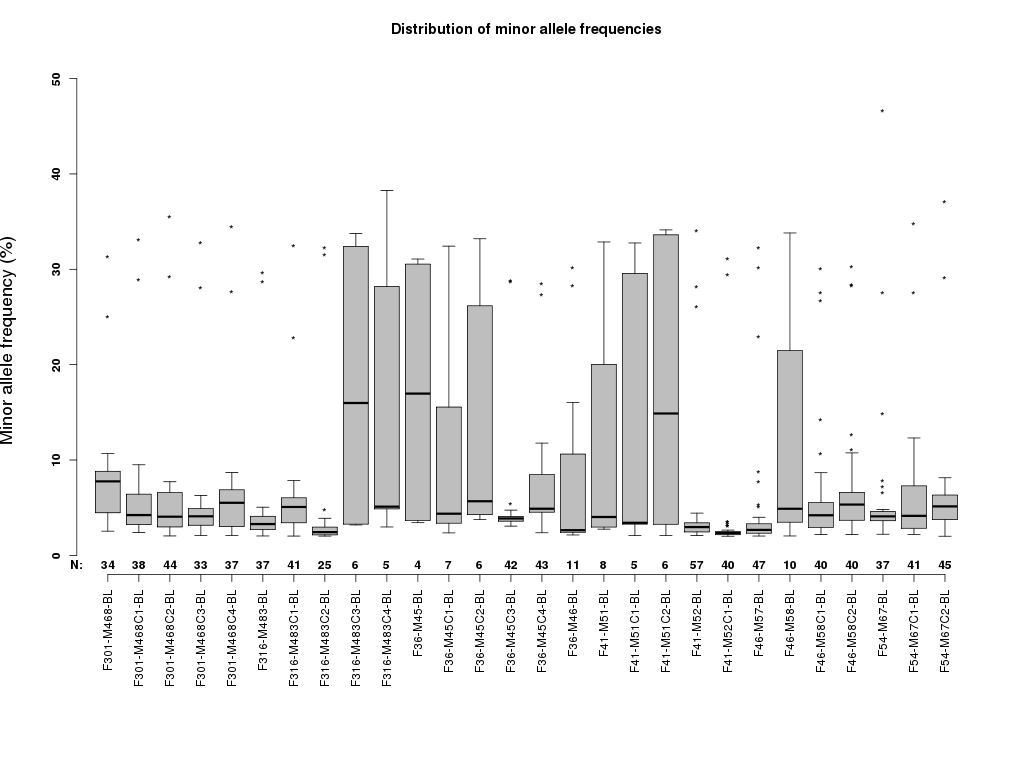
\includegraphics[width=1\textwidth]{images/galaxy-boxplot.png}
%    \caption[Galaxy Boxplot]{Galaxy Boxplot} 
%    \label{app:galaxy-boxplot}
%\end{figure}
The following listing represents the Pipeline for contamination detection defined in Cloudgene 
\begin{lstlisting}[caption={Cloudgene YAML file, defining the HaploChecker Workflow}, label=appyaml]

name: Contamination Check
description:  Check for Contamination
version: 0.1
website: 
category: mtDNA

cluster:

  image: us-east-1/ami-da0cf8b3
  type: m1.large,m1.xlarge
  ports: 80,50030,50070
  creationOnly: false
  installMapred: true
  initScript: install.sh
  service: hadoop
 
mapred:

  steps:
 
    - name: Create HaploGrep Inputfile
      jar: heteroplasmy-check-1.0.jar
      params: --input $input2 --output ${haplogrepInput}.txt

    - name: Haplogroup Contamination Check
      jar: haplogrep.jar
      params: --in ${haplogrepInput}.txt --out ${haplogroupsCheck}.txt --phylotree 16

    - name: Report Creation
      rmd: report.Rmd
      output: ${report}.html
      params: ${haplogroupsCheck}.txt

  inputs:
    - id: input2
      description: Input File
      type: local-folder

  outputs:

    - id: haplogrepInput
      description: Haplogrep Input File
      type: local-file
      download: true

    - id: haplogroupsCheck
      description: Detected Haplogroups Contamination with HaploGrep
      type: local-file
      download: true

    - id: report
      description: Contamination Report
      type: local-file
      download: true 
\end{lstlisting}

% \begin{figure}[!ht]
%     \centering
%     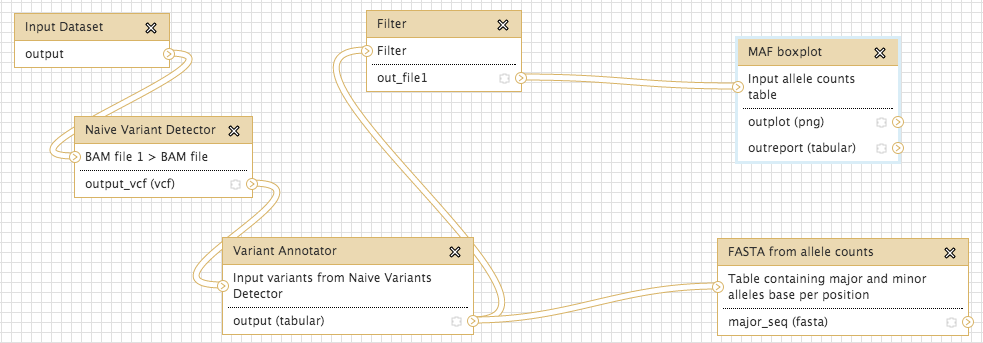
\includegraphics[width=1\textwidth]{images/galaxy-workflow-contamination.png}
%     \caption[Galaxy Workflow for Contamination estimation]{Galaxy Workflow for Contamination estimation} 
%     \label{app:galaxy-workflow}
% \end{figure}


\begin{figure}[!ht]
    \centering
    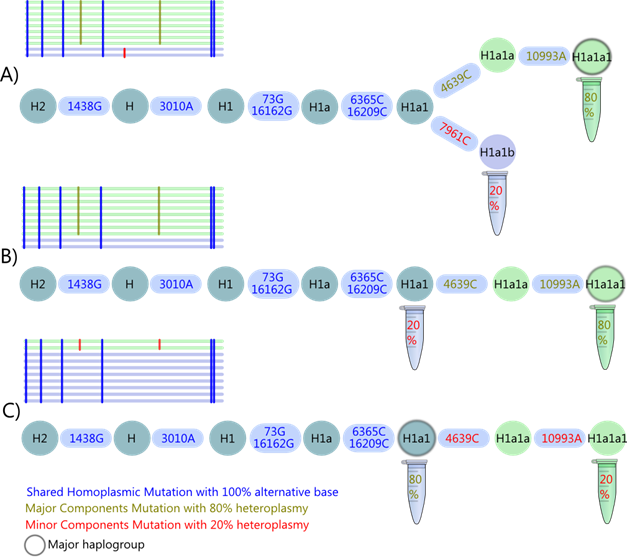
\includegraphics[width=1\textwidth]{images/heteroplasmy.png}
    \caption[Display of all possible pairwise sample contamination]{Display of all possible contaminations by pairwise comparison of major/minor haplotype within one analyzed sample. As an example a contamination level of 20\% over all reads is displayed. Shared polymorphisms of two haplotypes are presented in one branch, whereas the split into diverging branches evidences the two different lineage components (A). A mixture of two haplotypes within a single lineage but of different lineage depths (here minor H1a1 and major H1a1a1) is evidenced if no minor component can be found (B). A mixture of two haplotypes within a single lineage but of different lineage depths (here minor H1a1a1 and major H1a1) is evident if the minor components at equal levels lead to a meaningful haplogroup affiliation (C). Homoplasmic sites facilitate the identification of the branching pattern.} 
    \label{app:galaxy-boxplot}
\end{figure}